\documentclass[letterpaper,twocolumn,10pt]{article}
\usepackage{usenix2019,epsfig,endnotes}

% This is the setup file. It contains usepackage commands, acronyms, and other
% useful commands needed to set up the paper. Uncomment the relevant sections to
% use them.

% Packages. Make sure your LaTeX distribution actually has the packages!
\usepackage{acro}  % Acronyms
\usepackage{amsmath} % cases environment
\usepackage{color}  % Used to highlight comments
\usepackage{graphicx}  % To allow figures
\usepackage{msc}  % Message sequence charts
\usepackage{paralist}  % For tighter lists
\usepackage{xspace}  % For spacing after user-defined commands and others.
\usepackage[hyphens]{url}  % To make URLs display correctly in citations. The
                           % hyphens option allows line breaks after hyphens.
\usepackage{hyperref}  % Hyperlinks in citations and references


% Acronym definitions (requires acro package)

\DeclareAcronym{ca}{
  short={CA},
  long={certificate authority},
  long-plural-form={certificate authorities},
  alt={certification authority},
}
\DeclareAcronym{crl}{
  short={CRL},
  long={certificate revocation list},
}
\DeclareAcronym{ct}{
  short={CT},
  long={Certificate Transparency},
}
\DeclareAcronym{hsts}{
  short={HSTS},
  long={HTTP Strict Transport Security},
  short-indefinite={an},
  long-indefinite={an},
}
\DeclareAcronym{https}{
  short={HTTPS},
  long={HTTP over TLS},
  short-indefinite={an},
  long-indefinite={an},
}
\DeclareAcronym{mitm}{
  short={MITM},
  long={man-in-the-middle},
  short-indefinite={an},
}
\DeclareAcronym{mmd}{
  short={MMD},
  long={maximum merge delay},
  short-indefinite={an},
}
\DeclareAcronym{name}{
  short={CTAPS},
  long={Certificate Transparency with Automated Policies and Signaling},
}
\DeclareAcronym{oid}{
  short={OID},
  long={object identifier},
  short-indefinite={an},
  long-indefinite={an},
}
\DeclareAcronym{pki}{
  short={PKI},
  long={public-key infrastructure},
}
\DeclareAcronym{sct}{
  short={SCT},
  long={signed certificate timestamp},
  short-indefinite={an},
}
\DeclareAcronym{sth}{
  short={STH},
  long={signed tree head},
  short-indefinite={an},
}
\DeclareAcronym{tls}{
  short={TLS},
  long={Transport Layer Security},
}
\DeclareAcronym{x509}{
  short={X.509},
  long={X.509 Version 3},
  short-indefinite={an},
  long-indefinite={an},
}

% Example acronym definition. Uncomment to use.
%\DeclareAcronym{pki}{
  %short={PKI},
  %long={public-key infrastructure},
  %%short-plural={s},  % default
  %%long-plural={s},  % default
  %%long-plural-form={},  % use for irregular plurals
  %%short-indefinite={a},  % plural
  %%long-indefinite={a},  %plural
  %%alt={},  % alternate form
  %%alt-indefinite={a},
  %%short-format={},  % formatting for first short use
  %%long-format={},  % formatting for first long use
  %%first-long-format={\capitalisewords},  % must use mfirstuc package
  %%pdfstring={},  % string to use with hyperref section headings, etc.
%}



% User-defined commands go here.

\newcommand{\steve}[1]{\textcolor{magenta}{[SM: #1]}}
\newcommand{\draft}[1]{\textcolor{blue}{[Draft text: #1]}}
\newcommand{\emxs}[1]{\ensuremath{#1}\xspace}

\newcommand{\evidence}{\emxs{E}}
\newcommand{\hashfunc}{\emxs{H}}
\newcommand{\nodehash}{\emxs{h}}
\newcommand{\regstr}{\emxs{S}}

%\newcommand\definitionautorefname{Definition}
\renewcommand*{\equationautorefname}{Equation}
\renewcommand*{\figureautorefname}{Figure}
\renewcommand*{\sectionautorefname}{Section}
%\renewcommand*{\itemautorefname}{Definition}
\let\subsectionautorefname\sectionautorefname
%\newcommand{\algorithmautorefname}{Algorithm}



\setmsckeyword{}


% Fix ugly citation style: [1],[2] --> [1,2]

%\usepackage[noadjust]{cite}
%\renewcommand{\citepunct}{, }
%\renewcommand{\citedash}{--}

% Compression tricks - use if we need more space.

%\geometry{tmargin=.7in,bmargin=.7in,lmargin=.7in,rmargin=.7in}
%\renewcommand{\baselinestretch}{0.99}

% Aggressive space hacks. Use only in case of emergency!
%\usepackage[font=footnotesize]{caption}
%\usepackage{titlesec}
%\titlespacing\section{0pt}{5pt plus 1pt minus 0pt}{1pt minus 1pt}
%\titlespacing\subsection{0pt}{4pt plus 2pt minus 0pt}{1pt minus 0pt}
%\titleformat{name=\section}{\fontsize{11.7pt}{14pt}\bfseries}{\thesection}{1em}{}
%\titleformat{name=\subsection}{\fontsize{10.73pt}{12.87pt}\bfseries}{\thesubsection}{1em}{}
%\usepackage[final,babel,step=1,stretch=30,shrink=40]{microtype}
%\usepackage[all=normal,lists,paragraphs,wordspacing,leading]{savetrees}


\begin{document}

% USENIX: don't want date printed
\date{}

% USENIX: make title bold and 14 pt font (Latex default is non-bold, 16 pt)
\title{
  \Large \bf
  CAPS: Smoothly Transitioning to a More Resilient Web PKI
}
\author{
  Submission \#379
}

\maketitle

\subsection*{Abstract}
\steve{TODO}


\section{Introduction}
\label{sec:intro}

%Some questions to think about:
%\begin{compactitem}
%\item How can we move toward a world in which domains use multiple independent
  %certificate chains?
%\item How do we validate a self-signed certificate?
%\item What does it mean to have trust agility?
%\item Does the use of multiple independent certificate chains provide better
  %security and agility?
%\end{compactitem}

\acs{https}, built on \ac{tls}~\cite{rfc5246} and the Web \ac{pki}, lies at the
heart of secure end-to-end communication on the Web. \Acp{ca}, who vouch for the
binding between a domain's name and its public key, play a critical role in the
Web \ac{pki}. \Iac{ca}'s failure to correctly sign this binding in the form of a
public key certificate can lead to \iac{mitm} attack, allowing an adversary to
intercept and modify all communication between a client and domain. Recent years
have seen a plethora of these failures, both
accidental~\cite{sleevi2015sustaining} and
intentional~\cite{valsorda2015komodia}.

The failures of \acp{ca} continually remind us of the weakest-link security of
the Web \ac{pki}: a single misbehaving \ac{ca} can expose a domain to \ac{mitm}
attacks. Because we cannot prevent \acp{ca} from misissuing certificates,
protecting clients from these \ac{mitm} attacks entails making the \ac{pki}
resilient to certificate misissuance by enabling clients to detect and reject
misissued certificates. However, only domains themselves can with certainty
identify certificates misissued in their name. Clients therefore need a way to
determine a domain's \emph{certificate policy} (i.e., criteria for which
certificates the clients should consider correctly issued).

So far, proposed systems for communicating policy information to clients have
not gained traction in practice. These systems introduce additional trusted
parties~\cite{kim2013accountable} or assume that the entire Web will increase
its security at once~\cite{basin2014arpki}. These shortcomings motivate the
problem of designing a simple and deployable policy mechanism that requires
minimal effort from domains. \steve{The last part isn't motivated well; it would
  be nice if we could show that most policies are overkill for preventing
\ac{mitm} attacks that could have resulted from recent \ac{ca} failures.}

%The Web's \ac{pki} enables client browsers to authenticate the public keys of
%the domains they communicate with, and together with the \ac{tls}
%protocol~\cite{rfc5246} allows a client and domain to establish an end-to-end
%secure communication channel through \acs{https}. In the Web \ac{pki},
%trusted third parties called \emph{\acp{ca}} vouch for the binding between a
%domain's name and its public key. The correct operation of \acp{ca} are critical
%to the security of the Web \ac{pki}, and failures can lead to the client
%establishing a secure channel with the wrong domain. In some cases this
%scenario can lead to a \emph{\ac{mitm} attack}, in which even though the
%confidentiality and integrity guarantees of communication over \ac{tls} hold,
%they provide no benefit because an adversary is impersonating the client and
%domain to each other and can read and modify all communication between them.

%While there are many proposals (enumerated in \autoref{sec:related}) to fix the
%Web \ac{pki} by deterring, preventing, or recovering from \ac{ca} misbehavior,
%Google's \emph{\ac{ct}} system~\cite{rfc6962} has recently emerged as a widely
%deployed example of such a system, being scheduled for full deployment in
%October 2017. \ac{ct} does not prevent \ac{mitm} attacks, but rather enables
%widespread detection of \ac{ca} misbehavior. In \ac{ct}, a set of \emph{public
%logs} maintain a database of certificates they have observed (primarily sent to
%them by the \acp{ca} themselves) and provide cryptographic proofs called
%\emph{\acp{sct}} that show when these certificates were submitted to the log.
%Clients do not accept certificates unless they are sent with a requisite number
%of these \acp{sct}, ensuring that an adversary cannot use an unauthorized
%certificate for \ac{mitm} attacks without first exposing that certificate to the
%world.

%However, \ac{ct} has several notable shortcomings. \ac{ct} does not make
%\ac{mitm} attack prevention an explicit goal, but specifies the behavior of
%\emph{monitors}, who periodically download newly logged certificates and check
%for suspicious certificates. However, only domains know which certificates they
%have authorized, and \ac{ct} does not allow domains to check logs for
%certificates issued in their name. This disparity means that some manual effort,
%on the part of the monitors, domains, or both, is required to prevent \ac{mitm}
%attacks that result from unauthorized certificates. Both monitors and domains
%face hurdles due to this manual effort.

%With the increasing deployment of \ac{https} through certificate services such
%as Let's Encrypt,\footnote{\texttt{https://letsencrypt.org/}} monitors may not
%be able to keep up with the number of suspicious certificates that require
%further manual investigation. Previous work enables domains to alleviate this
%pressure on monitors by explicitly supplying \emph{policies} that specify
%criteria that a domain's certificates should meet, but it is not clear that the
%expressiveness of these policies and the burden they impose on domain operators
%is worth the benefit of protecting them from common certificate misissuances. We
%therefore seek a simpler, more automated system for specifying certificate
%policies through the \ac{ct} infrastructure. In particular, we aim to move
%towards \iac{pki} in which one-off mistakes by \acp{ca} do not expose domains to
%\ac{mitm} attacks.

Unfortunately, even with such policies, we still fall short of a truly secure
\ac{pki}. Domains may not only have different policies, but some domains may not
have policies at all because they do not deploy \ac{https}. Because we
realistically expect a world of partial deployment in which the set of deploying
domains increases incrementally over time, we need a mechanism to inform clients
\emph{when} to expect a certificate policy, not just \emph{what} policy to
expect. Moreover, this mechanism must be external to the Web \ac{pki} because it
indicates certification in the Web \ac{pki} itself. We call the problem of
designing such a mechanism the \emph{signaling} problem.

%These policies only exist for domains that actually deploy \ac{https};
%therefore, an adversary can bypass these protections by convincing the client
%that the target domain does not deploy \ac{https} at all (e.g., by blocking
%connections to port 443 over which domains usually serve \ac{https}). We
%therefore need a \emph{signaling} mechanism that securely indicates whether or
%not the client should expect the domain to deploy \ac{https}. Some existing
%approaches are opt-in, meaning that domains must explicitly register for these
%mechanisms, and thus only provide signaling for some sites (e.g., popular
%sites). Furthermore, the opt-in process is prone to misconfigurations, such as
%domains accidentally signaling that a subdomain deploys \ac{https}, thus
%rendering that part of the site inaccessible to clients. Other approaches
%require clients to perform online checks, degrading connection latency. Is it
%possible to improve on these approaches by reducing the action required by
%domains and by broadening the scope of domains that can signal \ac{https}
%deployment \emph{without} significantly increasing connection latency?

Existing approaches to the signaling problem
(\autoref{sec:background:signaling}) suffer from critical shortcomings. Some
require domains to opt in using a process prone to misconfiguration, and render
the domain inaccessible if misconfiguration occurs. Approaches that store
deployment information locally only signal \ac{https} deployment in a subset of
sites due to storage costs, and approaches that rely on external information
incur significant latency penalties and introduce additional trusted parties. We
therefore observe the need to address the signaling problem with a solution that
allows clients to confidently distinguish a site that deploys \ac{https} without
imposing performance penalties or trust assumptions.

To address the problems of managing certificate policies and of signaling
\ac{https} deployment in a simple and practical manner, we propose \ac{name}, a
system that \steve{gradually} increases the resilience of the Web \ac{pki}
against misbehaving \acp{ca}. \ac{name} leverages Google's
\ac{ct}~\cite{rfc6698} infrastructure, which relies on \emph{public logs} that
maintain a database of all issued certificates in the Web \ac{pki}.
%Because all certificates must be publicly logged to be accepted in Chrome
%browsers starting in October
%2017,\footnote{\url{https://cabforum.org/2016/10/19/2016-10-19-20-f2f-meeting-39-minutes/}}
\ac{name} repurposes these logs to also maintain certificate policies. \ac{name}
also achieves simplicity of policies by only tracking the number of \ac{ca}
certificates for a given key a client should expect. This simple approach also
means that for the vast majority of cases, domains do not need to change they
way they obtain certificates, and in fact only requires domains to occasionally
fetch information from a public log.

\ac{name} uses data from \ac{ct} logs and from Censys~\cite{durumeric2015search}
scans of \ac{https} sites to provide a complete view of all sites deploying
\ac{https}. Using data from these sources also means that domains do not have to
opt in to signal \ac{https} deployment. By using finite state methods and data
compression techniques, \ac{name} can also succinctly encode the set of sites
deploying \ac{https} to achieve fast, local signaling with efficient updates and
minimal additional connection latency.

In summary, this paper makes the following contributions:
\begin{compactitem}
\item It leverages \ac{ct} to propose a simple, deployable, and automated
  mechanism for maintaining and disseminating domain certificate policies.
\item It leverages finite state automata and data compression to present  a
  succinct design for communicating the set of sites deploying \ac{https}.
\item It shows through a comparative evaluation that \ac{name} requires only
  \steve{} extra communication, \steve{} additional storage, and \steve{}
  additional latency.
\end{compactitem}

%The Web \ac{pki} has seen several important improvements in recent years.
%\steve{Summary of CT, CAA, DANE, CAge, CRLite}

%Because \acp{ca} are trusted parties in the \ac{tls} \ac{pki}, they can enable
%\ac{mitm} attacks if they misbehave. Unfortunately, they have done so multiple
%times over the years, due to social engineering
%attacks~\cite{microsoft2001erroneous}, network breaches~\cite{comodo2011fraud,
  %hoogstraaten2012black}, operational errors~\cite{zusman2009sub,
  %langley2013enhancing, somogyi2015improved, sleevi2015sustaining}, or malicious
  %intent~\cite{percoco2012clarifying, langley2013further,
  %langley2015maintaining}. While in many cases the rogue certificates were
  %quickly detected and revoked, in some cases the certificates were actually
  %used in the wild in \ac{mitm} attacks~\cite{nightingale2011diginotar}. These
  %attacks are particularly noxious because the victim website may never find out
  %that it is being impersonated. Indeed, we have seen instances of targeted
  %attacks using fake certificates to impersonate websites to specific groups of
  %users~\cite{eckersley2011syrian}.

%While many attempts have been made to detect and prevent \ac{ca} misbehavior,
%one of the most widely-deployed fixes is \ac{ct}~\cite{rfc6962}. The goal of
%\ac{ct} is to enable fast and widespread detection of certificate issuance by
%publicly logging all certificates in \ac{tls}. A set of \emph{public logs}
%record all issued certificates in an append-only, tamper-proof fashion, and
%clients only accept a \ac{tls} certificate if it has been logged, thus forcing a
%potential adversary to publicize a certificate (making it detectable) before
%mounting a \ac{mitm} attack. However, simply adding logs to the existing
%\ac{tls} has several critical shortcomings. In particular, we identify three
%flaws with the current log-based architecture.


%a domain is associated with a policyin order to connect securely, a client needs
%to make sure that
%the policy was logged and registered (presence)
%the policy has not been updated since the value being read (recency)
%the policy was registered by the real domain (authenticity)

%what is the bad thing of having an incorrect policy?
  %accept too few certs or certs signed by the wrong ca (aka atker controlled)

%authenticated key-value store



\section{Background and Related Work}
\label{sec:background}

In this section, we describe relevant background and related work. We first
provide background on Merkle hash trees and \acl{ct}, both of which we refer to
in the remainder of the paper. We then discuss related work from both the
academic literature and projects from the industry and open-source communities
and their shortcomings. We then examine previous work that has addressed the
problem of specifying or inferring a domain's certificate policy. We conclude by
examining work that has addressed the problem of signaling HTTPS deployment in
domains.

\subsection{Merkle Hash Trees}
\label{sec:background:mht}

\begin{figure}
  \centering
  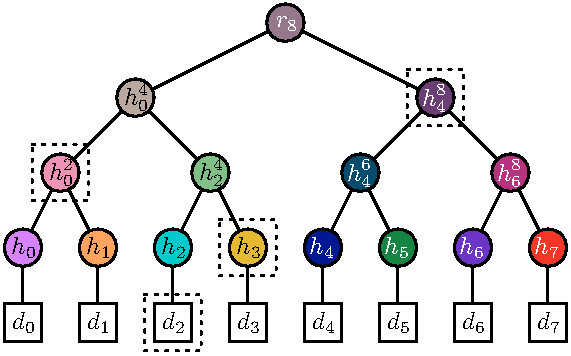
\includegraphics[width=\linewidth]{fig/mht-audit}
  \caption{Sample Merkle hash tree with eight leaf nodes. Dashed boxes indicate
  the nodes sent to prove the presence of the leaf $d_2$ in the tree.}
  \label{fig:mht-audit}
\end{figure}

A \emph{Merkle hash tree} is a binary tree in which each leaf node's value
represents data and each non-leaf node's value is the hash of its children's
values~\cite{merkle1988digital}. As shown in \autoref{fig:mht-audit}, the
structure of a Merkle hash tree allows one to efficiently prove that a data item
is present in the tree. Specifically, given the value of the root node of the
tree, one can verify the presence of any leaf node in the tree by computing a
number of hashes that is logarithmic in the number of data items in the tree.

A Merkle hash tree can store any number of nodes, i.e., the tree does not need
to be balanced. While several ways of computing the hashes in a non-balanced
tree exist, in this paper we use the method used in \ac{ct}~\cite{rfc6962}.
Specifically, given $n$ items in the Merkle hash tree, let \hashfunc be a hash
function, $d_i$ the $i$th data item (indexed from 0), and $a$ and $b$ integers
such that $0 < a < b \le n$. Then the hash of a non-leaf node representing the
$a$th to the $(b-1)$th data items is defined as
\begin{equation}
  \nodehash_a^b =
  \begin{cases}
    \hashfunc(0 \| d_a) & \mathrm{if\ } b = a + 1 \\
    \hashfunc(1 \| \nodehash_a^k \| \nodehash_k^b) & \mathrm{otherwise}
  \end{cases}
\end{equation}
where $\|$ denotes concatenation and $k = a + 2^{\lceil \log_2(b-a) \rceil - 1}$
(the largest power of 2 strictly less than $b - a$). For convenience, if $b = a
+ 1$ we write the hash as $\nodehash_a$ and call this a \emph{leaf hash}, and if
$a = 0$ and $b = n$ then we write the hash as $r_n$ and call this the \emph{root
hash}.

\begin{figure}
  \centering
  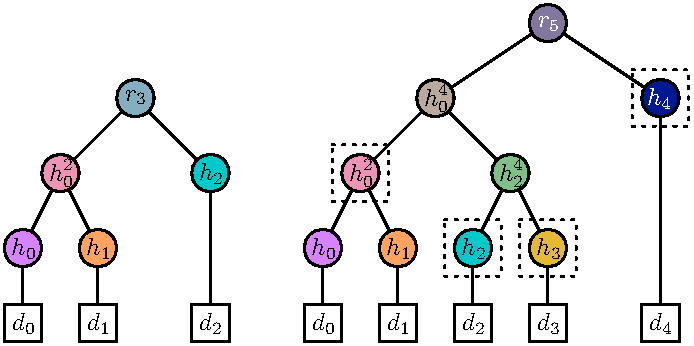
\includegraphics[width=\linewidth]{fig/mht-consistency}
  \caption{Sample Merkle hash trees with three and five data items,
  respectively. Dashed boxes indicate the nodes sent to prove consistency
between the root hashes $r_3$ and $r_5$.}
  \label{fig:mht-consistency}
\end{figure}

A Merkle hash tree can be used to implement an append-only, tamper-proof
log~\cite{crosby2009efficient}. As stated above, a Merkle hash tree can provide
an efficient \emph{proof of presence} for a given data item in the tree, thus
proving that an item was logged. To prove that the log is append-only, that is,
that no items have been changed or removed from the log, we can also use a
Merkle hash tree to provide an efficient \emph{proof of consistency} that is
logarithmic in the current size of the tree. As shown in
\autoref{fig:mht-consistency}, a proof of consistency allows one to compute the
root hash at two different times, thus showing that nodes have only been added
to the tree. A tamper-proof log would periodically sign and broadcast its root
hash, allowing clients to verify that it is not tampering with previously logged
data.

\subsection{Certificate Transparency}
\label{sec:background:ct}

\begin{figure}
  \centering
  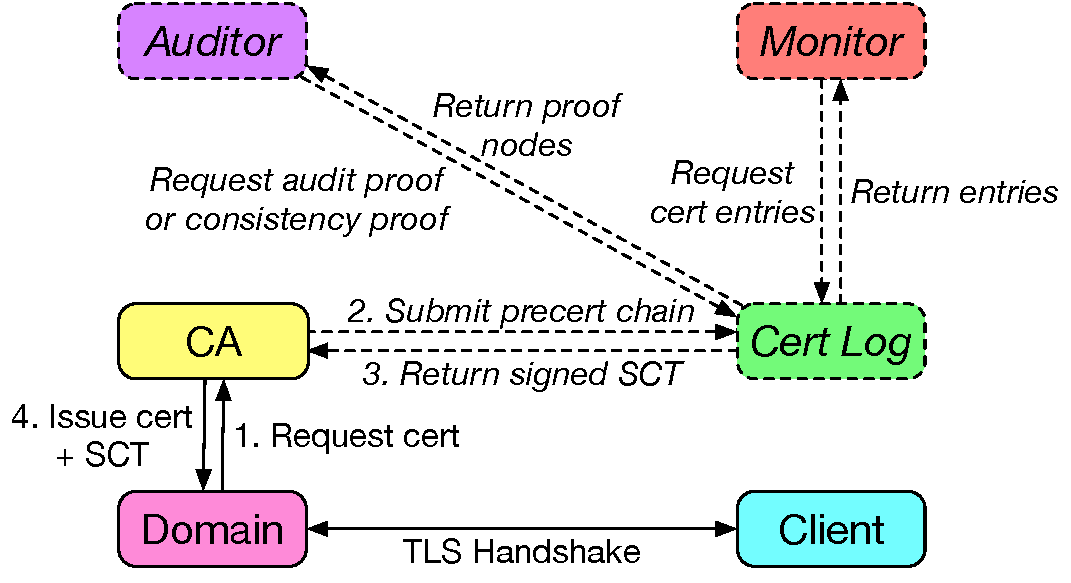
\includegraphics[width=\linewidth]{fig/ct}
  \caption{One possible configuration of the \ac{ct} architecture. Numbered
  steps denote the certificate issuance process. Dashed lines and boxes denote
entities or functions introduced by \ac{ct}, with their descriptions in
italics.}
  \label{fig:ct}
\end{figure}

\acf{ct} is a project by Google focused on enabling widespread detection of
certificate issuance~\cite{rfc6962}. As shown in \autoref{fig:ct}, \ac{ct}
introduces several new roles to the \ac{ca}-based ecosystem. \emph{Certificate
logs} are entities who record \ac{ca} behavior by maintaining a publicly
auditable, append-only, tamper-proof database of certificates. \emph{Monitors}
periodically retrieve these certificates to check for suspicious \ac{ca}
behavior, such as an obscure \ac{ca} issuing a certificate for Google.
\emph{Auditors} check for correct log behavior by periodically asking for
\emph{audit proofs}, which show that one or more certificates are in a log
database, or \emph{consistency proofs}, which show that the existing database
has not been tampered with, i.e., that no certificate has been changed, deleted,
or retroactively added to the log database.

A log leverages Merkle hash trees to implement its certificate database. As
explained above, the use of a Merkle hash tree allows a log to provide efficient
proofs of presence (i.e., audit proofs) and proofs of consistency (i.e.,
consistency proofs). While anyone may submit a certificate to a log, in current
practice \acp{ca} usually log certificates during the issuance process, as
depicted in \autoref{fig:ct}. Because attempting to update the Merkle hash tree
in real time may delay or block the certificate issuance process, logs define a
\emph{\ac{mmd}}, a time period after which a certificate is guaranteed to be
logged, and instead return a \emph{\ac{sct}}, which is effectively a promise to
add the certificate within the \ac{mmd}. The \ac{sct} is embedded into the
\ac{ca}-issued certificate as an X.509 extension and used to signal that a
domain uses \ac{ct} and that its certificate has been logged. Alternately, the
domain can send extra information such as \acp{sct} or audit proofs in the
\ac{tls} handshake using a \ac{tls} protocol extension.

%\draft{Monitoring and auditing details. Monitors periodically downloads all new
  %entries and verifies consistency proof. Does not need to keep cert entries
  %after finishing. Auditors periodically query for random audit proofs or
  %consistency proofs. Specifically, can pass a cert hash and a size of the tree
  %and get an audit proof in return, or pass two sizes of the tree and get a
  %consistency proof in return. To verify this information, log also provides a
  %function to get the latest signed tree head. In order to detect
  %\emph{equivocation} (i.e., showing different versions of the log to different
  %queries), auditors must gossip tree heads. The log's public key is known
  %through a trusted entity such as Google.}

%\draft{\ac{ct} does not check for revocation, though multiple extensions
%designed to handle revocation have been proposed (see \autoref{sec:related}).
%Perhaps the easiest way to do to this is to create a new Merkle hash tree every
%\ac{mmd} that contains as its leaves the list of \emph{currently valid}
%certificates.}

\subsection{Specifying and Inferring Domain Policy}
\label{sec:background:policy}

Previous work has proposed the use of domain-specified policies to protect
against \ac{mitm} attacks. In AKI~\cite{kim2013accountable} and its successor
ARPKI~\cite{basin2014arpki}, these policies are embedded within the certificates
themselves and specify attributes such as trusted \acp{ca} and public logs as
well as a ``cool-off period'' that forces potentially malicious certificates to
be visible in logs for some period of time before client can accept them. In
PoliCert~\cite{szalachowski2014policert}, the policies are stored separately in
logs. Other work, such as Blockstack~\cite{ali2016blockstack} or
IKP~\cite{matsumoto2017ikp}, has proposed placing policy information into a
blockchain. While IKP's policies operate similarly to those of PoliCert,
Blockstack simply provides the domain's keys directly. Of these proposals, only
ARPKI leverages the relationship between \acp{ca} and logs to ease the burden on
the domain during certificate issuance, but all proposals require the domain to
specify its policy in detail to prevent \ac{mitm} attacks resulting from
misbehaving \acp{ca}.

There has also been some work that takes a heuristic approach, using the past
behavior of \acp{ca} in order to determine how clients should trust them. For
example, CAge~\cite{kasten2013cage} propose a system that displays a browser
warning to users for certificates whose names are under a DNS top-level domain
that the issuing \ac{ca} has never signed for before. Perl, Fahl and Smith
propose to outright remove root certificates that have not been used to sign
(either directly or through \ac{ca} delegation) any observed certificates in the
past~\cite{perl2014you}. Both of these proposals use data from
Censys~\cite{durumeric2015search} or its predecessors, but do not use any
information from the domains themselves. Because of this, these approaches may
encounter situations where they mistake a legitimate, domain-initiated change
with an attempted \ac{mitm} attack and thus block a user from visiting a benign
site or expose a user to the \ac{mitm} attack. Indeed, a previous study of
changes in the Web \ac{pki}'s trust graph suggests that legitimate changes and
attacks share properties to the point that they cannot be easily
distinguished~\cite{amann2013no}.

\subsection{Signaling \ac{https} Deployment}
\label{sec:background:signaling}

Although \ac{hsts}~\cite{rfc6797} enforces the use of \ac{https} for a site
after a client has connected with that site over \ac{https} for the first time,
previous work has acknowledged the difficulty (in terms of both storage and
latency overhead) of identifying \ac{https}-deploying domains before the first
visit. The prevailing solution among browser vendors is \emph{\ac{hsts}
preloading}~\cite{keeler2012preloading}, in which browser vendors include a list
of the most popular sites that have deployed \ac{https}. These lists are
incomplete (covering only \steve{TODO: fill in} names in Chrome), and domains
must explicitly opt into adding themselves. As indicated by vendor-provided
guidelines,\footnote{\url{https://hstspreload.org/}} this process is prone to
mistakes by domain operators that lead to site inaccessibility.

As described in \steve{TODO: refer to previous section if mentioned elsewhere},
most approaches to disseminating certificate revocation information fail for
signaling because they rely on assumptions that do not hold in the signaling
problem. In particular, the use of \acp{crl}~\cite{rfc5280} does not scale to
the number of \ac{https}-deploying sites because we cannot assume that the
number of sites deploying \ac{https} will remain small compared to the overall
number of sites. More efficient versions of \acp{crl} also do not work: an
approach similar to Chrome's CRLsets~\cite{langley2012revocation} suffers from
the same incompleteness and opt-in hurdles mentioned above, and an approach
similar to CRLite~\cite{larisch2017crlite} relies on knowledge of all domain
names, which is infeasible in today's DNS due to many country code top-level
domains keeping their registries private. Approaches such as storing data in a
2-3 tree~\cite{naor1998certificate} or aoptimized Merkle hash
tree~\cite{laurie2012revocation}, while able to provide efficient proofs of
\ac{https} deployment, require online checks by clients, greatly increasing the
latency of connection establishment.

DANE~\cite{rfc6698}, which uses DNS to send a public key, certificate, or
\ac{ca} that the client should expect, can provide both signaling and policy
management with little added latency and without requiring browsers to store any
kind of signaling information. However, DANE relies on DNSSEC~\cite{rfc4033},
and both have a low deployment rate in today's
Internet,\footnote{\url{http://secspider.verisignlabs.com/stats.html}, retrieved
1 August 2017} with only 5,885 DANE records for \ac{https} and 1.67M verified
DNSSEC zones out of more than 329M names overall~\cite{dnib-14-1}. Changing
these numbers would require significant deployment efforts on the parts of
domains, including registering domain names through the subset of DNS registrars
that offer DNSSEC, usually as a paid service.


\section{CAPS Overview}
%\subsection{Overview}
\label{sec:design:overview}

\begin{figure}
  \centering
  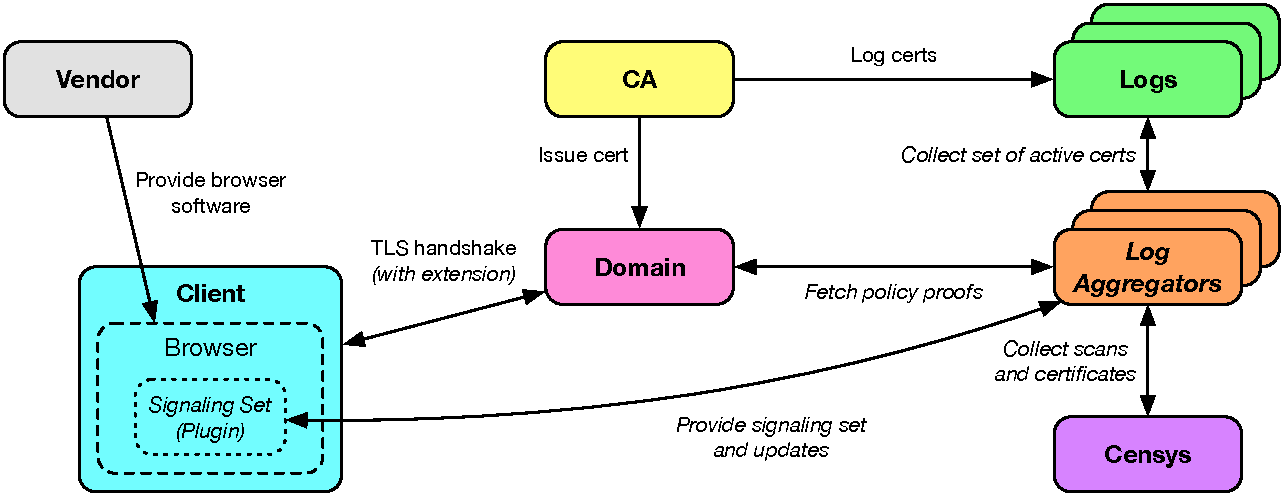
\includegraphics[width=\linewidth]{fig/arch}
  \caption{Overview of \ac{name} architecture (log auditors and monitors not
  shown). Dotted lines denote the browser and its components, and italic text
denotes new entities or actions in \ac{name}.  As shown in the diagram,
CAPS is currently implemented as a browser plug-in, but we envision it
would become a standard browser component.
  }
  \label{fig:overview}
\end{figure}

\paragraph{Goals}

\ac{name} primarily aims to enable a smooth transition from the Web's existing
\ac{pki} to an \emph{improved \ac{pki}} (which can range from an extension of
the existing \ac{pki} to a new \ac{pki} altogether). We assume that during this
transition, both the existing and improved \acp{pki} will coexist, and that the
improved \ac{pki} will make \ac{mitm} attacks more difficult to carry out.
Hence, \ac{name} must prevent downgrades to the old \ac{pki} as well as \ac{tls}
stripping. More precisely, if a client and server both support the improved
\ac{pki}, then when they perform a handshake, they should negotiate a session
key based on the domain's public key as certified in the improved \ac{pki}. As
secondary objectives, we also seek to prevent domains from becoming inaccessible
due to misconfiguration, private key loss, or private key compromise, and to
minimize the changes to existing interactions between clients, domains, and
\acp{ca}.

\paragraph{Adversary Model}

In designing \ac{name}, we consider a \iac{mitm} adversary. 
%We assume the adversary has access to the
%signing keys for $n$ \acp{ca} and can thus issue and revoke arbitrary
%certificates under these keys. 
We assume that the adversary has full
control of the network during the TLS handshake; that is, the adversary can
intercept, drop, or modify all messages sent among all entities described
below. We assume that the adversary cannot break standard cryptographic primitives.

\paragraph{Architecture}

\autoref{fig:overview} illustrates the \ac{name} architecture and how \ac{name}
achieves the goals stated above. Since \ac{name} transitions from the current
Web \ac{pki}, it necessarily includes the entities in the current \ac{pki}:
\begin{compactitem}
\item \emph{Domains} serve webpages to clients. Each domain has a name such as
  \texttt{example.com}.
\item \emph{\acp{ca}} issue certificates to domains. Each certificate binds a
  set of names to a single public key.
\item \emph{Clients} connect to domains over HTTP or \ac{https}, and in the
  latter case, verify the binding between a domain's name and public key.
\item \emph{Browser/OS vendors} (hereafter simply \emph{vendors}) provide the
  software by which clients connect to domains and verify domains' certificates.
\item \emph{Public logs} maintain a publicly auditable, append-only database of
  certificates, such as those used in \ac{ct}.
\end{compactitem}
\ac{name} introduces a new entity, the \emph{log aggregator}, a
high-availability entity that uses publicly available data to maintain a
database of domains that have deployed \ac{https} and/or the improved \ac{pki}.
As our figure shows, there may be multiple independent log aggregators. While
throughout this section we assume that the log aggregator is separate from other
entities and that there is a globally accepted set of known and trusted log
aggregators, in \autoref{sec:discussion} we discuss how we can relax these
assumptions, namely, by arguing that browser vendors should take on this
responsibility.

% Procedures from the current PKI
As shown in \autoref{fig:overview}, many of the interactions between entities in
the current \ac{pki} remain the same in \ac{name}. \acp{ca} remain entirely unchanged;
they issue certificates
to domains and log newly-issued certificates as they do in the current \ac{pki}
(with \ac{ct}). Clients and domains establish an encrypted communication channel
through the standard \ac{tls} handshake, and vendors provide clients with browser
software.

% Signaling set overview
To prevent an adversary from manipulating an attempted HTTPS connection into
an HTTP connection (and thus bypassing \ac{tls}
completely), the log aggregators use data from public logs to construct a
\emph{signaling set}, which succinctly represents the set of all domains that
support \ac{https}. The log aggregators build this set by downloading the set of
all currently valid (i.e., non-expired) certificates from the logs and
extracting all domains named in these certificates. The log aggregators then
make this set, as well as updates to this set over time, available to client
browsers.  When connecting to a server, the browser first checks whether
the server is in the signaling set; if it is, then the browser will refuse
to engage in an HTTP connection.

% Policy overview
To allow domains more control over their public keys than in the current
\ac{pki}, log aggregators use data from public logs to construct a set of
\emph{\ac{name} policies}, which allows each domain to establish one or more
\emph{authoritative public keys} in the \emph{current} Web \ac{pki}. \ac{name}
policies take a simple and intuitive approach: \emph{treat any public key backed
  by a maximal number of independent certificate chains\footnote{This term means
  that the certificate chains share no public keys except at the leaf.} in the
current \ac{pki} as authoritative}. A domain wanting to increase client
confidence in one of its public keys can obtain additional independent
certificates for that key, and the log aggregators will automatically update
their \ac{name} policies for that domain.

Intuitively, log aggregators simply provide signed pairs of the form
$(\hostname, \policy)$ where \hostname is a domain name and \policy is the
\emph{\ac{name} policy value}, i.e., the number of independent certificate
chains backing an authoritative key for \hostname. In case of a tie, \hostname
may have more than one authoritative key: if public keys $\pk_1$ and $\pk_2$ are
both backed by three independent chains then both public keys are treated as
authoritative for \hostname. To prevent an adversary from downgrading handshakes
in the improved \ac{pki} to a handshake in the existing Web \ac{pki}, each log
aggregator indicates which domains in its signaling set have a \ac{name} policy
value greater than 1.

When establishing an HTTPS connection with a server, clients can use the
signaling set to determine whether a domain has a \ac{name} policy value that is
exactly one or greater than one. In the former case, the client may connect to
the domain using the standard \ac{tls} handshake, but in the latter case, the
client requests policy information from the domain using a \ac{tls} extension
similar to ones currently under consideration for IETF 
standardization~\cite{rfc-extra-cert-1, rfc-extra-cert-2}.
Domains obtain the information from log aggregators and forward it to the
client; if a client receives and verifies a policy of $(\hostname, \policy)$, it
will expect to receive \policy independent certificate chains from the server.
If it receives fewer chains, or if any fail to validate, the client aborts
the connection.

The current PKI actually supports three classes of certificates: standard
domain-validated (DV) certificates, organization-validated (OV) certificates,
and extended validation (EV) certificates. EV certificates require domains to
undergo more rigorous screening than the other two. Hence, the actual \ac{name}
policy value is a pair $(\policy_{EV}, \policy_{!EV})$. For a given domain,
\ac{name} will treat as authoritative a public key with the largest observed
$\policy_{EV}$, with ties broken based on the largest value of $\policy_{!EV}$,
which represents the policy value of all non-EV certificates for the domain.


\section{CAPS Detailed Design}

In this section, we describe \ac{name} in detail, including how it signals which
domains have deployed \ac{https} and improvements to the Web \ac{pki}
(\autoref{sec:design:signaling}), how it provides stronger public-key
authentication over the existing Web \ac{pki} (\autoref{sec:design:policy}), and
how clients establish secure end-to-end connections with servers
(\autoref{sec:design:handshake}). We conclude by describing how \ac{name} thus
enables the bootstrapping of more advanced policies
(\autoref{sec:design:bootstrapping}).

\subsection{Building the Signaling Set}
\label{sec:design:signaling}

The signaling set represents
\begin{inparaenum}
\item a set of \acp{fqdn} (hereafter names) known to have deployed \ac{https}
  (by virtue of having a valid public-key certificate appear in a public log), and
\item the subset of names that have adopted \ac{name} (by
  virtue of having multiple independent certificate chains for the same public
  key).
\end{inparaenum}
Formally, the signaling set is a pair $(\httpsset, \multicertset)$ where
$\httpsset$ and $\multicertset$ are unordered sets of valid names in
ASCII\footnote{A valid name is a Unicode or ASCII string up to 253 bytes in
  length overall, with no label longer than 63 bytes~\cite{rfc1035}. We further
add the requirement that the name has \iac{tld} that is a current global
\ac{tld} according to ICANN. We use ASCII here because we can encode names in
Punycode.} and $\multicertset \subseteq \httpsset$. The set supports a query
operation, formally defined as $\query: \strings \to \{\nohttps, \onecert,
\multicert\}$ where $\strings$ is the set of all ASCII strings and \nohttps,
\onecert, and $\multicert$ are values indicating whether a string is a name
known to have no \ac{https} certificate, a public key backed by one certificate
chain, or a public key backed by multiple independent certificate chains,
respectively.
%Specifically, \query must satisfy \begin{align*} \query(\hostname) = \nohttps
%&\iff \hostname \notin \httpsset \\ \query(\hostname) = \onecert &\iff
%\hostname \in \httpsset \setminus \multicertset \\ \query(\hostname) =
%\multicert &\iff \hostname \in \multicertset \end{align*} for all $\hostname
%\in \strings$.

To build its signaling set, a log aggregator must first determine \httpsset
and \multicertset, which it can achieve using the set of all certificates in the
Web \ac{pki}. The log aggregator maintains a database of current certificates by
using information from public sources, namely,
\begin{inparaenum}
\item public logs that collect Web certificates 
  (e.g., CT and Censys -- see Section~\ref{sec:tracking}),
\item \acp{crl} such as those published by \acp{ca}~\cite{rfc5280} or browser
  vendors~\cite{langley2012revocation, goodwin2015revoking}, and
\item revocation information retrieved from OCSP responders~\cite{rfc6960}.
\end{inparaenum}
The log aggregator updates this database regularly (e.g., each day), thus
maintaining a list of certificates valid on a given day.\footnote{A certificate
  is valid on a given day if the signature on the certificate is valid and if
  that day falls in the certificate's validity period as defined by its
\texttt{notBefore} and \texttt{notAfter} fields~\cite{rfc5280}.}

The log aggregator extracts the names from the currently valid
certificates in its database;
%and converts internationalized domain names to ASCII using the IDNA conversion process~\cite{rfc5891}; 
the resulting set of distinct names is \httpsset. 
The log aggregator also analyzes the certificate chains
in this set to determine \multicertset, a procedure we describe in
\autoref{sec:design:policy}. The log aggregator then creates a representation of
the signaling set and makes it available to client browsers.

Because the signaling set must be available to each client that supports \ac{name},
%and may contain all names in DNS, 
the log aggregator must succinctly represent this set to minimize the bandwidth and storage burdens on
each client. However, simply minimizing the storage burden is insufficient;
clients must store the signaling set in memory to minimize connection latency
overhead. Thus the log aggregator must also represent this set in such a way
that clients can query the set with acceptably small latency and memory.

We considered several approaches when determining how to represent the signaling
set. A Bloom filter~\cite{bloom1970space} supports efficient set membership
queries, but has false positives (which for this application would result in
incorrectly flagging a site as under attack) and for the scale of data we
consider, results in too large a storage burden
(\autoref{sec:evaluation:https}). A filter cascade~\cite{salikhov2014using}
would eliminate false positives, but has the virtually impossible prerequisite
of knowing all names in the DNS namespace, which requires the cooperation of all
\ac{tld} operators (including many national governments). Finally, using an
existing data compression utility (e.g., zpaq) with aggressive compression
parameters could minimize the required storage space, but would also require
decompression and lookup each time a client tried to connect to a site whose
\ac{https} deployment status was not known, resulting in significant latency
overhead (\autoref{sec:evaluation:performance}).
%\steve{Distinguish transmission and local usage overhead}

%\begin{figure}
  %\centering
  %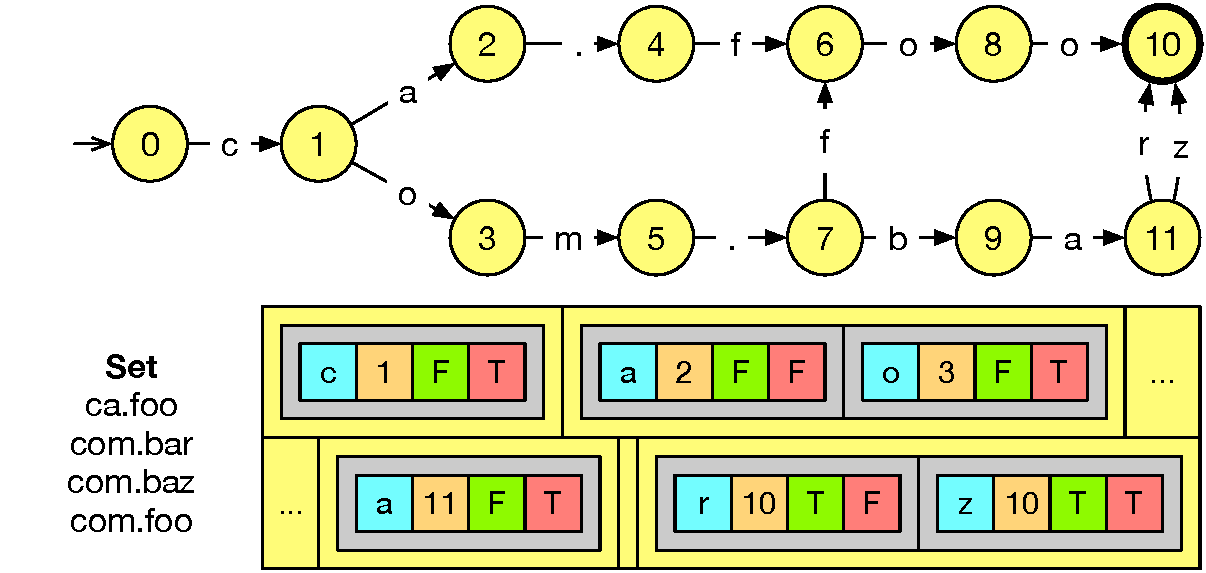
\includegraphics[width=\linewidth]{fig/dafsa}
  %\caption{A simple \ac{dafsa} with one-character transitions, along with the
    %set of strings it represents and its succinct representation as a vector of
    %variable-length bitstrings. In this representation, each edge (gray)
    %consists of a label (blue) and next state (orange), along with flags
  %indicating whether the next state is an accept state (green) and whether the
%edge is the last one outgoing from this state (red).}
  %\label{fig:dafsa}
%\end{figure}

\begin{figure}
  \centering
  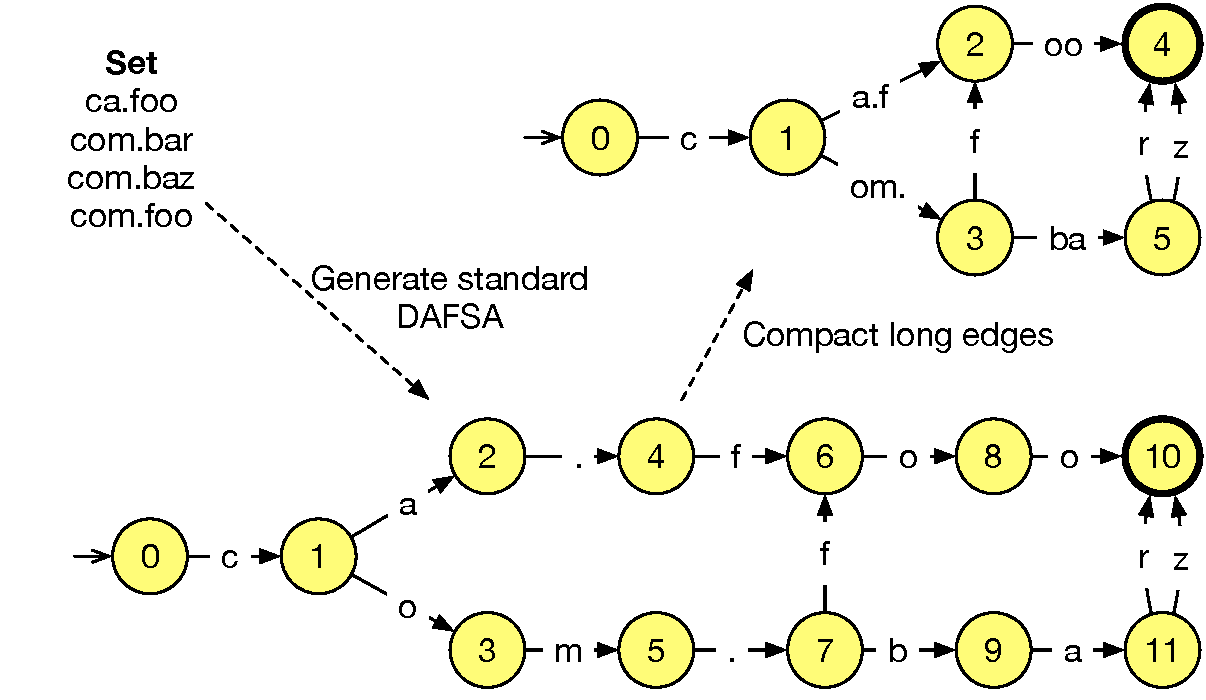
\includegraphics[width=\linewidth]{fig/dafsa_combined}
  \caption{The first stages of the \ac{dafsa} construction process used in
    \ac{name}. After generating the final \ac{dafsa} shown above, we use
    heuristic methods to generate a final \ac{dafsa} in a way that aims to
  minimize the size of the binary representation.}
  \label{fig:dafsa}
\end{figure}

In our log aggregator prototype, we ultimately chose to represent the signaling
set as a data structure known as a \emph{\acf{dafsa}}, which succinctly stores a
set of strings, supports efficient membership queries in this set, and supports 
efficient, compact construction~\cite{daciuk2000incremental}. As shown
in \autoref{fig:dafsa}, \iac{dafsa} takes advantage of both common prefixes and
suffixes that appear in a set of strings; since such patterns are frequent in a
large set of domain names, much of the redundancy in \httpsset can be removed with this
approach. Additionally, \acp{dafsa} can also be represented succinctly, using an
approach we summarize below~\cite{daciuk2012smaller}. Given the characteristics
of our input set as described in \autoref{sec:evaluation:implementation}, we
make an additional design change, \emph{path compaction},
to our \ac{dafsa} representation that further reduces its size.

\paragraph{Formal \ac{dafsa} Definition}

To precisely describe these changes, we begin by presenting a formal framework
to describe \acp{dafsa}. Formally, \iac{dafsa} is a tuple $(\symbols, \states,
\initstate, \transfunc, \finalstates)$ where
\begin{inparaenum}
\item \symbols is a set of possible \emph{input symbols},
\item \states is a set of \emph{states},
\item \initstate is an \emph{initial state} where $\initstate \in \states$,
\item $\transfunc: \states \times \symbols \to \states$ is a partial function
  called the \emph{state transition function} that maps a state-symbol pair to a
  new state, and
\item \finalstates is a set of \emph{accept states} where $\finalstates
  \subseteq \states$.
\end{inparaenum}
The \ac{dafsa} also has the restriction that the state transition function is
\emph{acyclic}, that is, there is no sequence of states and symbols $(s_1,
\ldots, s_n), (\sigma_1, \ldots, \sigma_n)$ where $\transfunc(s_i, \sigma_i) =
s_{i+1}$ for $1 \le i < n$ and $\transfunc(s_n, \sigma_n) = s_1$.

We represent queries to the signaling set within the \ac{dafsa} as follows: let
\symbols contain a unique symbol \multicertsymbol that is not present in any
name in \httpsset. Then, if there exists a sequence of
states and symbols $(s_0, \ldots, s_n), (\sigma_1, \ldots, \sigma_n)$ that
satisfies
\begin{inparaenum}
\item $\transfunc(s_i, \sigma_{i+1}) = s_{i+1}$ for each $i$ where $0 \le i < n$,
\item $\sigma_1 \| \dots \| \sigma_{n-1} = \hostname$, 
\item $\sigma_n = \multicertsymbol$, and
\item $s_n \in \finalstates$,
\end{inparaenum}
we say that $\query(\hostname) = \multicert$.
Otherwise, if
\begin{inparaenum}
\item $\transfunc(s_i, \sigma_{i+1}) = s_{i+1}$ for each $i$ where $0 \le i < n$,
\item $\sigma_1 \| \dots \| \sigma_{n} = \hostname$, and
\item $s_n \in \finalstates$,
\end{inparaenum}
then $\query(\hostname) = \onecert$. Otherwise, $\query(\hostname) = \nohttps$.

\paragraph{\ac{dafsa} Representation}

We begin by building the \ac{dafsa} as described in previous
work~\cite{daciuk2000incremental}. Though this previous work assumes transitions
based on a single character, we consider the possibility of multi-character
symbols and thus our symbol set consists of strings of length up to 253
characters:\footnote{Recall that DNS names can be a maximum of 253 characters.}
$\symbolstrings = \bigcup_{i=0}^{253} \symbols^i$, where \symbols is the set of
all ASCII characters allowed in domain names, and $\symbols^i$ indicates strings
of length $i$.

We succinctly represent this \ac{dafsa} as a bitvector by following the
high-level approach of previous work~\cite{daciuk2012smaller}. Intuitively, we
represent the \ac{dafsa} as a sequence of state encodings, which mostly consist
of outgoing transition encodings. By our definition of \transfunc, for a state
$s$, if $\transfunc(s, \sigma) = t$, then each outgoing transition must be
represented by an encoding of the label $\sigma$ and the destination state $t$.
We observe that in this construction, the overall number of outgoing
transitions, as well as the size of the representation of each transition's
label and destination state, strongly influence the size of the final bitvector.
We thus focus on leveraging patterns in the underlying data to minimize the
overall size of the \ac{dafsa} representation.

\paragraph{Path Compaction}

%\begin{figure}
  %\centering
  %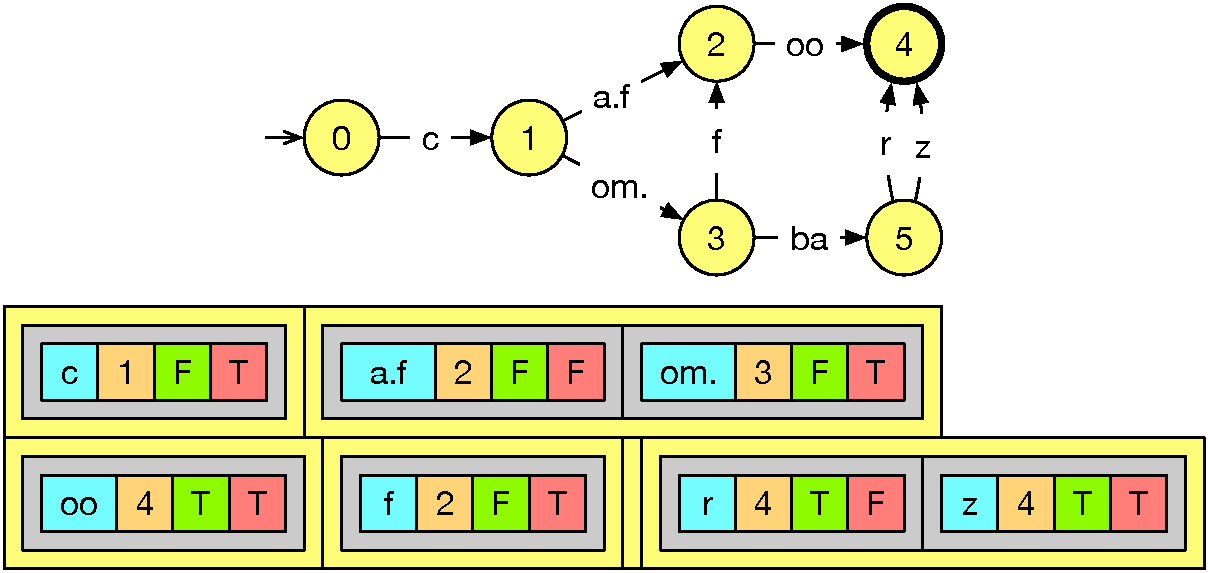
\includegraphics[width=\linewidth]{fig/dafsa_compact}
  %\caption{The \ac{dafsa} from \autoref{fig:dafsa} with its long edges
  %compacted. The binary representation is more succinct than its counterpart.}
  %\label{fig:dafsa_compact}
%\end{figure}

We extend the design of prior work with \emph{path compaction}, which
minimizes the \ac{dafsa} representation by reducing the overall number of
transitions. Intuitively, path compaction removes a connected set of states from
the \ac{dafsa} and replaces transitions into or out of this set with transitions
equivalent to paths through the set. As we formalize below, we can model this
process as the transformation of one \ac{dafsa} into another and use this model
to determine how we should select a set of nodes to ensure a minimal \ac{dafsa}
representation.

Given \iac{dafsa} $(\symbols, \states, \initstate, \transfunc, \finalstates)$,
we define a \emph{path} between $s_1$ and $s_m$ to be a sequence of alternating
states in \states and symbols in \symbols, written $(s_1, \sigma_1, \ldots,
s_m)$, where for all $i$ where $1 \le i < m$, $\transfunc(s_i, \sigma_i)
= s_{i+1}$.
We say that a set of states $\stateset
\subseteq \states$ is a \emph{connected component} if either $\stateset
\subseteq \finalstates$ or $\stateset \cap \finalstates = \emptyset$, and for
any two states $t, u \in \stateset$, 
any path between $t$ and $u$ contains only states in $\stateset$.
The \emph{upstream states} of a connected component \stateset, written
\upstream{\stateset}, is the set of all states $s \in \states \setminus
\stateset$ for which there exists a state $t \in \stateset$ and a symbol
$\sigma$ where $\transfunc(s, \sigma) = t$. The \emph{downstream states} of
\stateset, written \downstream{\stateset}, is the set of all states $s \in
\states \setminus \stateset$ for which there exists a state $t \in \stateset$
and a symbol $\sigma$ where $\transfunc(t, \sigma) = s$. A path \emph{through} a
connected component \stateset is a path $(s_1, \sigma_1, \ldots, s_m)$ where
$s_1 \in \upstream{\stateset}$, for all $i$ where $1 < i < m$, $s_i \in
\stateset$, and $s_m \in \downstream{\stateset}$.

Path compaction consists of repeatedly
\begin{inparaenum}
\item selecting a connected component \stateset within the \ac{dafsa},
\item calculating the estimated reduction in representation size from compacting
  the paths through \stateset, and
\item if the change reduces the size of the \ac{dafsa} representation, removing
  these states from \states and replacing the paths through \stateset with an
  equivalent set of transitions.
\end{inparaenum}
Specifically, when removing \stateset, we transform the \ac{dafsa} $(\symbols,
\states, \initstate, \transfunc, \finalstates)$ to $(\symbols, \states \setminus
\stateset, \initstate, \transfunc', \finalstates)$, where for all paths $(s_1,
\sigma_1, \ldots, s_m)$ through \stateset, $\transfunc'(s_1, \sigma_1 \| \dots \|
\sigma_{m-1}) = s_m$.

Our goal is to select components that result in the greatest reduction in size.
To determine the size reduction of removing a connected component, we must
consider both the reduction in the number of edges in the \ac{dafsa} as well as
any changes to the Shannon entropy of the distributions of symbols and
destination states in the \ac{dafsa}, as removing a component would cause these
distributions to change. To quantify this change, we define several helpful
variables.

For a set $X \subseteq\states$, let \numtrans{X} denote the set of transitions
that start or end in $X$, that is, the number of triples $(s, t, \sigma)$ where
$\transfunc(s, \sigma) = t$ and $s$ or $t$ (or both) is in $X$. For a connected
component $C$, let \numpaths{C} denote the set of paths through $C$. Then the
change in the number of edges by removing $C$ through path compaction is
$|\numpaths{C}| - |\numtrans{C}|$. By collecting the distribution of symbols in
\numtrans{S} and \numtrans{C}, as well as the concatenated symbols in
\numpaths{C} (which we can find via depth-first search from \upstream{C}), we
can compute the change in entropy in symbols and similarly for destination
states, which we write as \symboldh and \destdh, respectively. Suppose that we know the
original entropies \symbolh and \desth, and that we define $\dentropy = \symboldh +
\destdh$ and $\entropy = \symbolh + \desth$. Then we can compute the difference in
size between the two \acp{dafsa} as
\begin{equation}
  |\numtrans{S}| \dentropy + \left(|\numpaths{C}| - |\numtrans{C}|\right)
  (\entropy + \dentropy)
\end{equation}
and only remove $C$ if this quantity is negative.

We found several classes of components that, for our underlying set of domain
names, provided substantial reductions in the size of the \ac{dafsa}
representation. The first was to select what we call \emph{isolated paths}, that
is, paths of the form $(s_1, \sigma_1, \ldots, s_m)$ where for all $i$ such that
$1 < i < m$, $s_i$ only had one incoming and one outgoing transition. Using
techniques from prior work~\cite{daciuk2000incremental} to build the \ac{dafsa}
results in a significant number of isolated paths. Hence performing path
compaction on all such paths results in a size savings of nearly 10\% of the
original \ac{dafsa} size. We also found that selecting a constant $\alpha$ and
then selecting components consisting entirely of states that had one incoming
transition and $\alpha$ outgoing transitions (or vice versa) yielded more modest
but still nontrivial size reductions for $\alpha = 2$ and $\alpha = 3$.

\subsection{Building the \ac{name} Policy Database}
\label{sec:design:policy}

The \ac{name} \emph{policy database} represents a binding between a name and a policy, that
is, the number of independent certificate chains that a client
should expect during a handshake with a server corresponding to the name.
To construct and maintain this database, each log aggregator must keep track of
the certificates and chains active for a domain at any given time. The log
aggregators again rely on the data used to build the signaling set.
%from public sources for this information,
%which includes the data used to build the signaling set, as well as certificate
%chains observed by public logs.

\begin{figure}
  \centering
  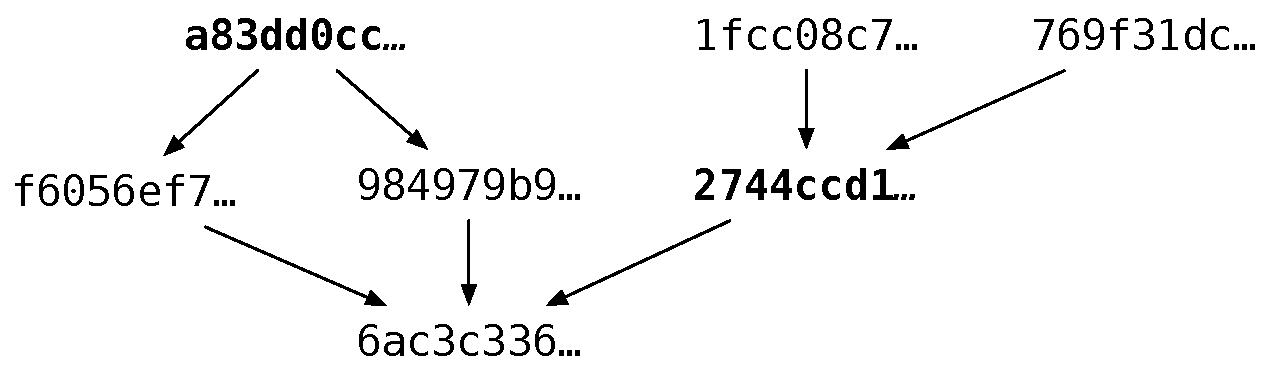
\includegraphics[width=0.9\linewidth]{fig/chain}
  \caption{Sample certificate fingerprint graph. $A \rightarrow B$ indicates
    that a certificate with fingerprint $A$ is the authority public key for a
    certificate with fingerprint $B$. Though the leaf certificate
    $\texttt{6ac3c336}\ldots$ has four chains, the bolded fingerprints show that
    only two of the chains are independent.}
  \label{fig:chain}
\end{figure}

A log aggregator uses this data to maintain an internal database with
(many-to-many) maps of
\begin{inparaenum}
\item certificates to names,
\item certificates to public keys, and
\item certificates to chains.
\end{inparaenum}
Regular updates to this database (described in \autoref{sec:design:signaling})
ensure that the log aggregator has a list of currently valid certificates. The
log aggregator can then use the database to construct a mapping of names to
policies. Specifically, the aggregator creates a graph of certificate
fingerprints as shown in \autoref{fig:chain}, and computes the \emph{policy
value}, the minimum number of \ac{ca} public keys that must be compromised for a
\ac{name}-enabled browser to accept a fraudulent certificate for this site. The
policy value can be computed using a straightforward approach (e.g., computing a
minimal vertex separator), allowing the log aggregator to easily construct a
mapping of certificate fingerprints to policy values. The log aggregator can
then perform a series of simple join operations to map each name to the maximum
policy number associated with a certificate containing the name.

The log aggregator constructs this name-to-policy mapping each time it receives
data from public sources (recall from \autoref{sec:design:signaling} that this
occurs at regular, scheduled intervals). Once it has created the mapping, the
log aggregator certifies the name--policy-value pairs in this mapping by
timestamping and signing them. For auditability, the log aggregators
can additionally take an approach similar to that of logs in \ac{ct}, using a
Merkle hash tree to store their policy proofs over time in a cryptographically
verifiable, append-only fashion.

With the policy databases of the log aggregators, a domain can provide the
information necessary for clients to establish the domain's authoritative public
key. The domain periodically downloads the latest \emph{policy proofs}, which
are signed and timestamped name-policy pairs, from each of the log aggregators.
For a name \hostname, a policy value \policy, a timestamp \timestamp, and a log
aggregator \logagg, we specify the policy proof to be
\begin{align}
  %data &= \logagg \concat \hostname \concat \timestamp \concat \policy \\
  \policyproof(\logagg, \hostname, \policy, \timestamp) &= 
  \left\{data, \signature(\pk_{\logagg}^{-1}, data)\right\} \mbox{ where}
  \nonumber \\
  data &= \logagg \concat \pk_{\logagg} \concat \hostname \concat \timestamp \concat \policy
\end{align}
where $\pk_{\logagg}$ and $\pk_{\logagg}^{-1}$ denote respectively the public
and private keys of \logagg, and $\signature(K, m)$ denotes a signature on $m$
with private key $K$. The domain uses these proofs in the handshake described
below.

\subsection{Connection Establishment}
\label{sec:design:handshake}

To establish a connection to a domain, a client (e.g., browser) first queries
the signaling set for the domain's name. If this query returns \onecert then the
client performs a standard TLS handshake (and refuses any attempts to downgrade
to plain HTTP). If the query returns $\multicert$, indicating the domain has
more than one certificate chain, then the client performs the \ac{name}-extended
TLS handshake to establish a connection with the domain. The result of the query
to the signaling set is cached until the next signaling set update, which
eliminates the need for this query in future connections. Caching is
particularly effective at minimizing overhead for operations such as session
resumption~\cite{rfc8446}.

The \ac{name}-extended TLS handshake protocol allows a client to verify a
domain's authoritative public key. The \ac{tls} handshake
protocol~\cite{rfc5246} provides support for open-ended extensions (implemented
in cryptographic libraries), and thus we designed our protocol as an extension
within the existing \ac{tls} handshake.

During the initial
  ClientHello message, the client includes a \ac{name} extension message, which
  consists of a single integer \numlas, indicating the number of policy proofs
  that the domain should send back.
%We assume that a reasonable maximum value for \numlas is enforced; for example,
  %a domain may abort the handshake if \numlas is beyond some acceptable
  %maximum.
In an initial deployment, we expect that typically $k=1$, but allowing the use
of larger values for $k$ provides resilience against compromised log
aggregators.  See Section~\ref{sec:analysis:weaknesses} for further discussion.

The domain then sends back a ServerHello message that contains \numlas recent
policy proofs from \numlas distinct log aggregators, as well as \numlas
certificate chains, which allows the client to verify the domain's policy value
and the certificate chains supporting this value. Formally, suppose a domain has
hostname \hostname and policy value \policy, and selects a set of log
aggregators $\{\logagg_1, \ldots, \logagg_\numlas\}$. Let $\policyproofshort_i =
\policyproof(\logagg_1, \hostname, \policy, \timestamp_i)$ for $1 \le i \le
\numlas$, where $\timestamp_i$ is the timestamp of the policy proof from
$\logagg_i$. Then, the domain sends the following back in the ServerHello
extension message:
\begin{equation}
  \{\policyproofshort_1, \ldots, \policyproofshort_\numlas, \certchain_1,
  \ldots, \certchain_{\policy - 1}\}
\end{equation}
where $\certchain_j$ is a certificate chain for \hostname. In the extension
message, the domain only sends $\policy - 1$ certificate chains because the
remaining chains will be sent in the ServerCertificate message of the TLS
handshake.

The client then checks that
\begin{inparaenum}
\item the signature on each policy proof is valid,
\item the timestamp for each policy proof is sufficiently recent,
\item the name in each policy proof matches the domain name to which 
      the browser is connecting,
\item the policy value for each policy is one more than the number of
  certificate chains sent in the domain's extension message, and
\item each certificate chain is valid as specified in the X.509v3
  standard~\cite{rfc5280}.
\end{inparaenum}
If the above checks pass, the client can then continue with the standard TLS
handshake, which requires the client to verify an additional certificate chain
in the ServerCertificate message and perform all other checks required by the
\ac{tls} handshake protocol.

While our current design uses a custom TLS extension, in the future, \ac{name}
may instead be able to leverage recently proposed TLS
extensions~\cite{rfc-extra-cert-1, rfc-extra-cert-2} designed to allow the
transmission of additional certificates (primarily to facilitate content hosting
by CDNs).  

\subsection{Bootstrapping Advanced Policies}
\label{sec:design:bootstrapping}

Once an authoritative public key for a domain has been established through the
\ac{name} handshake, signatures made by the corresponding private key are useful 
beyond simply improving the domain's security in the current \ac{pki}.
In particular, a signature from the authoritative public key can be
used to verify the binding between a domain and a richer set of policies. For
example, in systems such as ARPKI~\cite{basin2014arpki} and
PoliCert~\cite{szalachowski2014policert}, these policies can specify a set of
\acp{ca} that are authorized to issue certificate for the domain, or even make
the domain a \ac{ca} for itself by pinning specific public keys to the domain.
In this way, the authoritative public key established in \ac{name} can be used
to bootstrap confidence in these advanced policies while preventing downgrades
to the old \ac{pki}.

This bootstrapping approach obviates the need for logs to directly store the
policies, which can be quite large in these previously proposed systems.
Moreover, in \ac{name}, this bootstrapping can take place at any time during
deployment. This means that in the case of a lost private key, a domain can
simply obtain \policy new independent certificate chains, and in the case of a
compromised private key, $\policy + 1$ new independent chains. This contrasts
with previous proposals, which often rely on heavyweight processes that involve
manual \ac{ca} intervention.



\section{Analysis}
\label{sec:analysis}


\section{Evaluation}
\label{sec:evaluation}

\subsection{Signaling Mechanism}

We implemented our signal set in \steve{probably C++}. We first compare our
FSA-based approach to other methods, in particular, simply compressing the
signal set and the use of Bloom filters.

\steve{We first eliminated many compression algorithms from consideration by
  considering the Pareto frontier of the compressed size and the decompression
  time. We only compared the decompression time, not the full lookup time,
  because once the set is decompressed, it is the same regardless of compression
algorithm and we would expect the lookup times to be the same.}

We first ask simply how much space the compressed representation of the signal
set takes on disk. We compared 


\section{Discussion}
\label{sec:discussion}


\section{Conclusion}
\label{sec:conclusion}

\steve{TODO}


% USENIX: bibliography and endnote formatting
{\footnotesize \bibliographystyle{acm}
\bibliography{bib}}
\theendnotes

\end{document}
